\documentclass[14pt,letterpaper,norsk]{article}
\usepackage{babel}
\usepackage[T1]{fontenc}
\usepackage{extsizes}
\usepackage{graphicx}
\usepackage[bookmarks]{hyperref}
\usepackage{pdfpages}
\usepackage[lyric]{songs}
\usepackage[utf8]{inputenc}

\title{Sanghefte for Ifi-galla 2021}
\author{Cybernetisk Selskab}
\date{}

\setlength{\oddsidemargin}{0in}
\setlength{\evensidemargin}{0in}
\setlength{\textwidth}{6in}
\setlength{\topmargin}{0in}
\setlength{\topskip}{0in}
\setlength{\headheight}{0in}
\setlength{\headsep}{0in}
\setlength{\textheight}{9.1in}
\settowidth{\versenumwidth}{1.\ }
\pagestyle{empty}

\newindex{titleidx}{lbtitle}
\newauthorindex{authidx}{lbauth}
\newscripindex{scripidx}{lbscrip}

\begin{document}


\includepdf{forside.pdf}
\newpage



\begin{songs}{titleidx,authidx,scripidx}


\begin{intersong*}
{%
\parindent 0pt
\noindent
\ifx\preLilyPondExample \undefined
\else
  \expandafter\preLilyPondExample
\fi
\def\lilypondbook{}%
\input{4c/lily-838aca3c-systems.tex}
\ifx\postLilyPondExample \undefined
\else
  \expandafter\postLilyPondExample
\fi
}
\end{intersong*}
    
\beginsong{EN BAYER I HÅNDEN}

\beginverse
Jeg er født med en bayer i hånden,
sådan har jeg tenkt meg at jeg også ville dø -
Jeg drikker øl til jeg oppgiver ånden,
la døden komme langsomt av seg selv - pø om pø -
Men akkurat nå føler jeg meg frisk og sunn -
Helt i fra vuggen så suttet jeg på flasken,
jeg var atten før jeg fikk et bryst i min munn:
\endverse

\beginchorus
Jeg er født med en bayer i hånden,
sådan har jeg tenkt meg at jeg også ville dø.
Jeg drikker øl til jeg oppgiver ånden,
la døden komme langsomt av seg selv - pø om pø
\endchorus

\beginverse
I en kupe på expressen til Bergen,
sitter det en pikelill og piken vinder garn -
overfor henne der sitter det en herre,
han si'r hun er den fjerde han har sett er med et barn -
«Gud,» hviner piken, «hvem si'r jeg er gravid?»
«Rolig,» si'r mannen, «vi rekker nok det hele,
vi er først i Bergen om en halv times tid -»
\endverse

\beginchorus
Jeg er...
\endchorus

\beginverse
Den gamle soldat fikk et ben skutt av i krigen,
så kom han på sykehus et år det stakkars kre -
etter en tid kom de fram med målebåndet,
så fikk han et splitter nytt av ekte eketre -
Mannen så stolt på sitt nye ben og tenkte:
«Aj, så fantastisk , det beste ben jeg eier,
får jeg en åreknute høvler jeg den av -»
\endverse

\beginchorus
Jeg er...
\endchorus

\beginverse
Når jeg er død og er puttet ned i graven,
ja, da vil jeg håpe mine negler de vil gro -
Så vil jeg grave meg en gang under haven
hen til den nærmeste lendeveiskro -
Der vil jeg kjøpe en bayer eller to,
så vil jeg grave meg tilbake til graven,
der vil jeg nyte den i fred og i ro -
\endverse

\beginchorus
Jeg er...
\endchorus
\endsong






\begin{intersong*}
{%
\parindent 0pt
\noindent
\ifx\preLilyPondExample \undefined
\else
  \expandafter\preLilyPondExample
\fi
\def\lilypondbook{}%
\input{eb/lily-0ae6adec-systems.tex}
\ifx\postLilyPondExample \undefined
\else
  \expandafter\postLilyPondExample
\fi
}
\end{intersong*}

\beginsong{DET ER MEG DET SAMME HVOR VI HAVNER NÅR VI DØR}
\beginverse
Det er meg det samme hvor jeg havner når jeg dør
Det er meg det samme hvor jeg havner når jeg dør
For jeg har venner begge steder som vil motta meg med heder
Det er meg det samme hvor jeg havner når jeg dør
\endverse

\beginverse
Det e`kke sikkert vi får brennevin når vi dør
Det e`kke sikkert vi får brennevin når vi dør
Så la oss derfor drikke drammen nu i aften vi er sammen
Det e`kke sikkert vi får brennevin når vi dør
\endverse

\beginverse
Minst ett vertshus må der lukkes når jeg dør
minst ett vertshus må der lukkes når jeg dør
Jeg har slitt og jeg har slevet for å få det hele gjevet
minst ett vertshus må der lukkes når jeg dør
\endverse

\beginverse
Der blir ingen prestetaler når jeg dør
Der blir ingen prestetaler når jeg dør
jeg skal minnes ved et beger som en gammel skjørtejeger
Der blir ingen prestetaler når jeg dør
\endverse

\beginverse
Jeg vil spille med sankt Peter når jeg dør
Jeg vil spille med sankt Peter når jeg dør
Og hvis jeg spiller som jeg pleier, kan jeg loppe`n for en bayer
Jeg vil spille med sankt Peter når jeg dør
\endverse
\endsong

\beginsong{SKÅLEVISE 2}
\beginverse
Og dette skal være gratulanten sin skål, hurra
Ja, dette skal være gratulanten sin skål, hurra
Og skam for den som ikke, gratulanten sin skål vil drikke

(det drikkes)

Hurra, hurra, den skål den var bra, den skåler vi for, hurra!
\endverse
\endsong


\beginsong{LAMBO}
\beginverse
Alle: Se der sitter en fyllehund,
Mine herrer Lambo.
Sett nu glasset for din mund,
Mine herrer Lambo.
Se hvordan hver dråpe vanker
Nedad halsen på den dranker.
Lambo, Lambo,
Mine herrer Lambo.
\endverse

\beginverse
Den ene: Jeg mitt glass utdrukket har,
Alle: Mine herrer Lambo.
Den ene: Ei en dråpe finnes kvar,
Alle: mine herrer Lambo.
Den ene: Som bevis jeg nå vil vende
Glasset på dets annen ende.
Alle: Lambo, Lambo,
Mine herrer Lambo
\endverse

\beginverse
Alle: Han kunne kunsten,
Han var et jævla fyllesvin.
Så går vi til neste mann, og
ser hva han formår.
\endverse
\endsong

\beginsong{LILLE TORSTEIN}

\beginverse
Lille Torstein var fra Røa,
han var liten dum og stygg,
og de andre barna mobba'n så
han var jo aldri trygg.
\endverse

\beginverse
Sjebnen herjet med han ille,
toget gjorde kort prosess,
kjørte over begge beina
så han sto der kun til kness.
\endverse

\beginverse
Og på sykehuset sa de,
du vil aldri mere gå!
Og så lo de godt og moret seg
og lattern den var rå!
\endverse

\beginverse
Men da gikk han hen kastet seg
fra toppen av et fjell,
men det gjorde ingen ting,
for det ble jul alikevel!
\endverse
\endsong

\beginsong{FINSK DRIKKEVISE}
\beginverse
NU!
\endverse
\endsong

\beginsong{THEODOR}
\beginverse
Jeg elskede sjøen ifra jeg var ung
og svømmede rundt som en sei
fadriorei.
\endverse

\beginverse
En dag da jeg badet min velskapte kropp,
kun bagenden ragede opp,
fadriorei.
\endverse

\beginverse
:/:folk ropte:"Der svømmer en alligator!"
Så var det .... til - Theodor.:/:
\endverse
\endsong

\beginsong{SKÅLEVISE 2}
\beginverse
Og dette skal være gratulanten sin skål, hurra
Ja, dette skal være gratulanten sin skål, hurra
Og skam for den som ikke, gratulanten sin skål vil drikke

(det drikkes)

Hurra, hurra, den skål den var bra, den skåler vi for, hurra!
\endverse
\endsong

\beginsong{ØL ER BÅDE MAT OG DRIKKE}
\beginverse
Øl er både mat og drikke --- nektar og ambrosia.
Uten duger helten ikke, øl er derfor godt å ha,
øl er godt å ha, gjør deg sterk og glad
løft ditt glass og drikk, det er en gammel skikk,
det er en gammel skikk.
\endverse

\beginverse
Og når ølet ut er drukket fyller vi vårt glass på ny.
Inntil tørsten vel er slukket kan man intet bedre by,
intet bedre by, ølet har sitt ry
løft ditt glass og drikk, det er en gammel skikk,
det er en gammel skikk.
\endverse
\endsong

\beginsong{NU KLINGER IGJENNOM DEN GAMLE STAD}
\beginverse
Nu klinger igjennom den gamle stad på ny en studentersang,
og alle mann alle i rekke og rad svinger opp under begerklang,
og mens borgerne våkner i køia og hører det glade kang-kang,
stemmer alle mann, alle mann, alle mann, alle mann, alle mann, alle mann;
\endverse

\beginchorus
Studenter i den gamle stad ta vare på byens ry!
Husk på at jenter, øl og dram var kjempernes meny.
Og faller I alle mann alle, skal det gjalle fra alle mot sky:
La'ke byen få ro, men la den få merke den er en studenterby.
\endchorus

\beginverse
I denne gamle staden satt så mangen en konge stor,
og hadde nok av øl fra fat og piker ved sitt bord,
og de laga bøljer i gata når hjem i fra gilde de for,
og nu sitter de alle mann alle i Valhall og traller til oss i kor:
\endverse

\beginchorus
Studenter i den gamle stad .......
\endchorus

\beginverse
På Elgeseter var det liv i klosteret dag og natt:
Der hadde de sin kagge og der hadde de sin skatt.
De herjet i Nonnenes gate og rullet og tullet og datt,
og nu skuer de fra himmelen ned og griper sin harpe fatt:
\endverse

\beginchorus
Studenter i den gamle stad .......
\endchorus

\beginverse
Når vi er vandret hen og staden hviler et øyeblikk,
da kommer våre sønner og tar opp den gamle skikk:
En lek mellom muntre buteljer samt aldri så lit' erotikk.
Og så sitter vi i himmelen og stemmer opp vår replikk:
\endverse

\beginchorus
Studenter i den gamle stad .......
\endchorus

\endsong

\beginsong{SKÅL KAMERATER}

\beginverse
Skål, Kamerater!  
Godt humør,   
tidsnok kommer sorgen,  
full i dag, og full i går  
og også full i morgen!  
Ompa ompa drekk deg i hjæl!  
(blrurlrurb) SKÅL!!!  
\endverse

\endsong

\beginsong{OLE JOHAN}[by=Melodi: Ola Tveiten]

\beginverse
Eg heiter Ole Johan og eg er ein IT-mann
Eg eig ein PC og meg sjøl og gjer så godt eg kan
Og studentene dei progger og sliter seg i havn
Men eg stjeler bare kode, og endrer variabel-navn
\endverse

\beginchorus
Og koden blei lang og treig og støgg
-Sudelida sudelidei!
Den støggaste eg har sett
-Sudelida sudelidei!
Nei, det var bare spaghetti
Om ikkje han ikkje kjører til evig tid
Så skal eg eta opp lua mi
-Sudelida sudelidei! (Hei!)
\endchorus

\beginchorus
Tra la lalala la!
Fyll opp mitt tomme krus!
\endchorus

\beginverse
Og eg har vel koda java og eg har vel koda c
Og eg har vel lengta heim ein gong til senga og til fred
Og eg har vel budd på ifi i vekesvis i strekk
Og eg har vel banna om kvelden og ønska meg ti mil vekk.
\endverse

\beginchorus
men koden har ikkje kompilert
-Sudelida sudelidei!
Det var jævlig komplisert
-Sudelida sudelidei!
og retter sendte svar
fikk fristen utsatt av ein kar
I frå oktober til januar.
-Sudelida sudelidei! (Hei!)
Tra la lalala la
Fyll opp mitt tomme krus!
\endchorus

\beginverse
Og eksamen kjeme snart men redd det er eg ei
for eg har smiske med sensor, eg veit at han er grei
Og om eg skulle stryke, så bli eg ikkje lei
et nytt år på IFI, hipp hurra for meg
\endverse

\beginchorus
Så ropar dei alle høgt hurra
-Sudelida sudelidei!
kan ta flere verv da
Sudelida sudelidei!
Men tilslutt skal alt gå bra
en bachelorgrad det skal jeg ha
Nei, det blir nok ikke nav!
-Sudelida sudelidei! (Hei!)
Tra la lalala la!
Fyll opp mitt tomme krus!
\endchorus
\endsong
\beginsong{LEVE INFORMATIKKEN}[by=Melodi: Kalinka]

\beginverse
Leve informatikken
Den ække matte og fysikk
Lenker som bandt så hardt vårt store fag
Hyll, fagidd-joter, våre ledere!
\endverse

\beginchorus
Leve Newton, von Neumann og Turing og Knuth!
Leve Shannon og Wiener og Kalman og Gauss!
Leve Dijkstra, McCarty og Hopper og Hoare,
Runge-Kutta, Henrici, de Boor, Tsjebysjeff!
\endchorus

\beginverse
Hullkort-maskin for pionèrer,
Skrive-terminal so genèrer,
Nå vil vi minnes det som en gang var,
den gang vi sang i gledesrus:
\endverse

\beginchorus
Leve DEC-10 og Mycro, Nord-10 og Nord-12.
Leve Univac og Eniac og Illiac, Balrog!
Leve Cyber og Burroughs, Amdalh, IBM,
Wegematic og Nusse og CD og MIX!
\endchorus

\beginverse
Puncher og skrivere skranglet
Skjermer hadde ikke samme mangler
Så la oss hylle terminalene
Det er som vi aldri hadde andre enn dem:
\endverse

\beginchorus
Leve Tandberg, Tektronix, Dec-scope, Infoton!
Leve Beehive og Silent, Display, Teletype!
Leve Alnabru, Diablo, Titt-titt, Linjegods!
Leve Tandberg, og Tandberg og Tandberg, Tandberg!
\endchorus

\beginverse
Nå har vi X-terminaler,
Mac-er som synger og taler,
Skriker til maskinen, men får ikke svar,
Hyll, fagidd-jotter, så maskinene!
\endverse

\beginchorus
Leve Sun-er og SPARC-er og DECstation, Mac,
Leve Tandberg og Quadra, Atari og Next,
Leve Indy og SE og Convex og Vax,
og en PC, Toshiba, DEC-20 og Perq
\endchorus

\beginverse
Taster i vei på mitt manus,
Word eller Frame eller Cranus,
Nettverk' er nede, så nå gir jeg opp,
Disken er full og min tanke tom
\endverse

\beginchorus
Leve Unix og Simula og Emacs og X,
Leve \LaTeX{} og Beta og Emacs og C,
Leve QWERTY og WYSIWYG og Emacs og \TeX{},
og ESCAPE eller mus med et klikk, og klikk-klikk
\endchorus

\beginverse
Fest på informatikken
Dosent og student vanker sammen
Det er ikke hver dag vi har tid til slikt
Men la nå dette bli en tradisjon
\endverse

\beginchorus
Leve Madsen og Hurlen og Lyche og Dahl!
Leve Spurkland og Reenskaug og Nygaard og Maus!
Leve Winther og Bjerknes og Hisdal, Wang!
Leve Hesjedal og Kirkerud og OLE JOHAN!!!!!!
\endchorus
\endsong

\end{songs}

\newpage

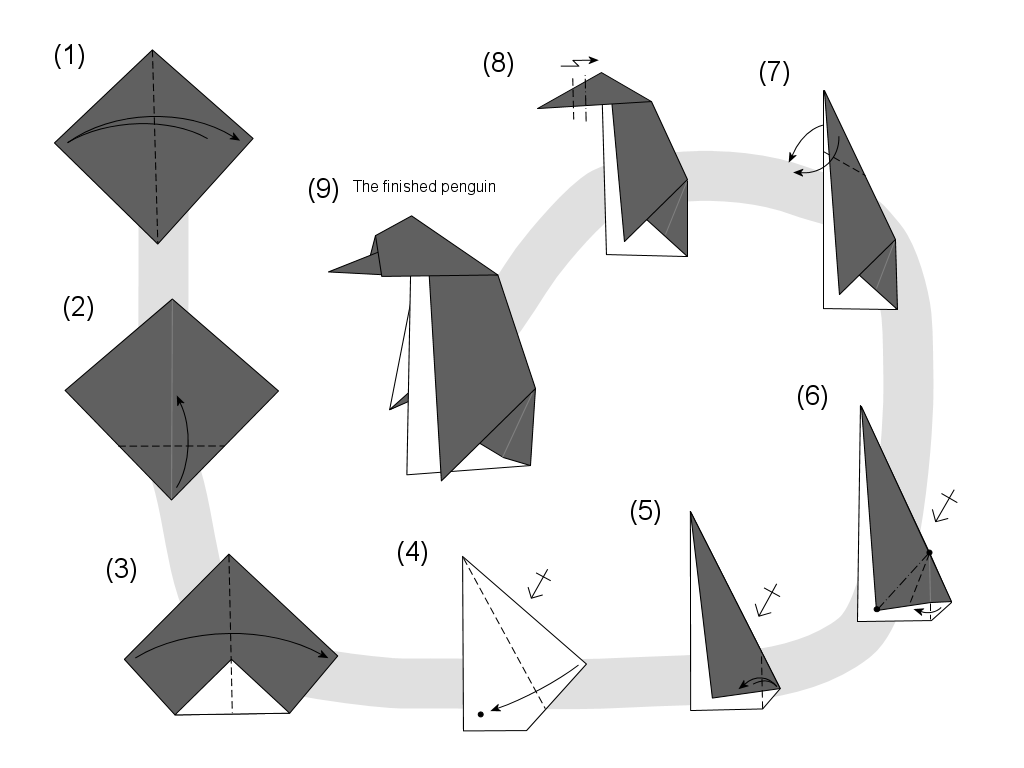
\includegraphics[width=\textwidth]{penguin_diag.png}

\end{document}